\slajdid{02-s040}
\begin{frame}[t,label=02-s040]
\gusttekst
Uočite da smo na primer Tabelu sa 3 promenljive, mogli da zamislimo i u 3D prostoru kao preklapanje dve tabele

\begin{columns}[c,onlytextwidth]
\begin{column}{.35\textwidth}\centering
\input{slike/tikz/s040_tabela_2x4.tex}
\end{column}
\begin{column}{.08\textwidth}\centering \(=\)\end{column}
\begin{column}{.50\textwidth}\centering
% C=1 namerno zadržava oznake A=1,0 iz originala, uz indekse 4,5/6,7.
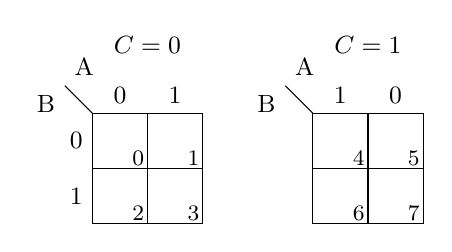
\begin{tikzpicture}[font=\fontsize{9}{10}\selectfont,x=7mm,y=7mm,baseline=(current bounding box.center)]
\draw (0,0) rectangle (2,2) (1,0)--(1,2) (0,1)--(2,1);
\draw (0,2)--(-.5,2.5) node[above right] {A} node[below left] {B};
\node[above] at (.5,2) {0};\node[above] at (1.5,2) {1};
\node[left] at (0,1.5) {0};\node[left] at (0,.5) {1};
\node[above] at (1,2.9) {\(C=0\)};
\foreach \x/\y/\lab in {1/1/0,2/1/1,1/0/2,2/0/3}{
 \node[anchor=south east,inner sep=1pt,font=\fontsize{8}{9.5}\selectfont] at (\x,\y) {\lab};
}
\draw (4,0) rectangle (6,2) (5,0)--(5,2) (4,1)--(6,1);
\draw (4,2)--(3.5,2.5) node[above right] {A} node[below left] {B};
\node[above] at (4.5,2) {1};\node[above] at (5.5,2) {0};
\node[above] at (5,2.9) {\(C=1\)};
\foreach \x/\y/\lab in {5/1/4,6/1/5,5/0/6,6/0/7}{
 \node[anchor=south east,inner sep=1pt,font=\fontsize{8}{9.5}\selectfont] at (\x,\y) {\lab};
}
\end{tikzpicture}

\end{column}
\end{columns}

\begin{columns}[c,onlytextwidth]
\begin{column}{.29\textwidth}
Jasno je da su sada gledajući u 3D preklapanje, kao što smo već rekli susedna polja 0 i 4, 1 i 5 itd\ldots\ Prema tome pravilna površina 1.og reda je i površina koja prekriva polja 0 i 4
\end{column}
\begin{column}{.19\textwidth}\centering
\input{slike/tikz/s040_povrsina_prvog_reda.tex}
\end{column}
\begin{column}{.29\textwidth}
ili pravilna površina 2.og reda je i površina koja prekriva polja 0, 1, 4 i 5.
\end{column}
\begin{column}{.19\textwidth}\centering
\begingroup
\fontsize{20}{22.2}\selectfont
\renewcommand{\small}{\fontsize{20}{22.2}\selectfont}
\mbox{\scalebox{.45}{%
\begin{karnaugh-map}(label=middle)[2][4][1][$A$][$B$][$C$]
\foreach \x/\y/\lab in {1/3/0,2/3/1,1/2/2,2/2/3,1/1/6,2/1/7,1/0/4,2/0/5}{
 \node[anchor=south east,inner sep=2pt,font=\fontsize{17.78}{19.8}\selectfont] at (\x,\y) {\lab};
}
\implicantedge{0}{1}{4}{5}
\end{karnaugh-map}}}
\endgroup

\end{column}
\end{columns}
\end{frame}
